% Constructing a Benchmark When Every Component Is a Language Model.
% Track B methodology paper. arXiv preprint format (single column).
% Self-contained: all figures are TikZ / pgfplots, no external image files.
%
% Every number here traces to a committed artifact; the mapping is asserted by
% tests/test_pipeline_paper.py.

\documentclass[11pt]{article}

\usepackage[margin=1.1in]{geometry}
\usepackage[T1]{fontenc}
\usepackage{lmodern}
\usepackage{microtype}
\usepackage{amsmath}
\usepackage{amssymb}
\usepackage{booktabs}
\usepackage{array}
\usepackage{caption}
\usepackage{enumitem}
\usepackage{tikz}
\usepackage{pgfplots}
\usepackage[hidelinks]{hyperref}

\pgfplotsset{compat=1.18}
\usetikzlibrary{positioning, arrows.meta, fit, backgrounds,
decorations.pathreplacing, calc}

\captionsetup{font=small, labelfont=bf, width=.95\textwidth}

\renewcommand{\topfraction}{0.92}
\renewcommand{\bottomfraction}{0.8}
\renewcommand{\textfraction}{0.07}
\renewcommand{\floatpagefraction}{0.8}

% Tufte-leaning plot defaults, identical to the dataset paper's: no frame, no
% grid, minimal ticks. Every rule that survives is carrying information.
\pgfplotsset{
tufte/.style={ axis lines=left, axis line style={draw=black!55, line
width=.4pt}, tick style={draw=black!55, line width=.4pt}, tick align=outside,
label style={font=\small}, tick label style={font=\footnotesize}, legend
style={draw=none, fill=none, font=\footnotesize}, every axis plot/.append
style={line width=.9pt}, }, }

\definecolor{ink}{gray}{0.15}
\definecolor{mid}{gray}{0.50}
\definecolor{pale}{gray}{0.78}
\definecolor{accent}{RGB}{176,48,36}

\newcommand{\code}[1]{\texttt{\small #1}}

% Zenodo deposit identifiers, minted 2026-09-19. \zenodoDOI is this paper's
% CONCEPT DOI, which resolves to the latest version: v1 (22838603) carried an
% error in 5.2 and v2 corrects it, so page one must not point a reader back at
% v1. \companionDOI is the dataset and validity paper's. Both are pinned by
% tests/test_pipeline_paper.py, so a mistyped or invented identifier cannot ship.
\newcommand{\zenodoDOI}{10.5281/zenodo.22838602}
\newcommand{\companionDOI}{10.5281/zenodo.22838321}

\title{\textbf{Constructing a Benchmark When Every\\Component Is a Language Model}\\[.35em]
\large An engineering account, and five model dependencies we could not
remove}
\author{Mehul Srivastava\\\normalsize Independent researcher\\
\normalsize ORCID: \href{https://orcid.org/0009-0008-1031-304X}{0009-0008-1031-304X}}
\date{19 September 2026\\[.45em]
\normalsize DOI: \href{https://doi.org/\zenodoDOI}{\zenodoDOI}}

\begin{document}
\maketitle

\begin{abstract}
\noindent A synthetic benchmark built today runs language models at nearly
every stage. One model writes the world, another authors the items, a third
performs the task, a fourth scores the output, and a fifth is often asked
whether the fourth can be trusted. Each use makes the measurement a function
of a model, and a benchmark is only as reproducible as the least pinned model
in its pipeline. This paper is the engineering account of one such pipeline,
built end to end and shipped. We removed some of those model dependencies by
construction. Others we could only pin. The rest we could only measure and
disclose.

The governing rule is that no language model decides what is true. A hidden
ledger of typed, tiered, timestamped facts induces a computable expected belief
state $B(p,t)$. The generator's model writes prose around those facts and has no
authority over them. The criteria an output is scored against are derived from
$B$, drafted under a fixed prompt and validated mechanically against the ledger
rather than read off any output. A model still decides
whether a given output satisfies a fixed criterion, and \S6.3 is what that
costs. Every item ships with a
counterfactual twin whose stream is byte-identical except for the probed fact,
and credit requires both sides to behave correctly, which makes an item
self-falsifying. No item is assumed to measure anything until a memoryless
worker has failed it and a fact-injected worker has passed it.

The architecture removes the model from truth and from nowhere else, and the
residue is measurable. Item validity is a property of
the item \emph{and} the worker. Under identical rules, 37 of 54 probe clusters
survive the ceiling gate for one model and 17 of 54 for a smaller sibling. The
harness counts as part of the worker. Identical weights behind two agent
scaffolds agree on 65\% of twin-ceiling outcomes against a prespecified 90\%
bar. The judge fails by criterion kind rather than in aggregate,
over-accepting on every absence-phrased error and under-accepting on every
scope error, which cancels to a 14--14 split that reads as unbiased noise; the
automated audit meant to catch this contained no absence-phrased criteria and
could not have failed. A four-model judge panel, set beside the committed
judge as a fifth rater, agrees across all ten rater pairs at $\kappa$
0.93--0.97 and with a human at 0.52--0.56 in every one of the five
comparisons, and majority, unanimous-AND and unanimous-OR aggregation all
score at or below the best single judge. The
pinned worker was then deprecated by its provider mid-study, which turned
re-anchoring from a paragraph in a maintenance plan into a procedure we had to
run.

We report the apparatus that caught these alongside the apparatus that did
not: four prespecified bars that failed and are carried as failures; a
scorer-exploit audit that failed its own literal bar; and a detector layer
built, measured at zero true positives across 19 honest flips, and discarded
the same day.
\end{abstract}

\begin{center}
\begin{minipage}{0.93\textwidth}
\small\noindent\textbf{Keywords:} benchmark construction; synthetic data
generation; LLM-as-judge; judge validity; inter-rater reliability; agent
evaluation; reproducibility.
\end{minipage}
\end{center}

\begin{center}
\begin{minipage}{0.93\textwidth}
\rule{\textwidth}{0.4pt}\\[0.55em]
\small\noindent\textbf{How to read this paper.} This is a construction
method and its cost, not a benchmark result. No comparative result between
memory systems appears anywhere;
the evaluation that would have produced one was cancelled by the deprecation
in \S6.5.
\\[0.55em]\rule{\textwidth}{0.4pt}
\end{minipage}
\end{center}

\section{Introduction}

\subsection{The pipeline is the instrument}

Benchmarks used to be data. A researcher collected examples, wrote an answer
key, and the answer key was the instrument; if you disagreed with a label you
could look at it and argue. Synthetic benchmarks for agents are not like that.
The examples are generated, the answer key is often generated, the task is
performed by a model, and the output is scored by a model because the output
is a paragraph of prose rather than a class label. What used to be a dataset
is now a pipeline, and the pipeline is the instrument.

This changes what reproduction means. A dataset reproduces by being
downloaded. A pipeline reproduces only if every model in it is pinned, and
only for as long as those models exist. Neither condition holds by default,
and the second one stopped holding for us on 2026-09-04, when the provider
deprecated the worker our entire valid set had been screened against. The
standards literature asks a benchmark to document its construction, its
statistics and its validity argument \cite{betterbench, abc, construct}. A
pipeline has to document its models too, and a deprecation date it does not
control.

We built memory-bench, a benchmark for how agent memory systems handle
organizational knowledge, over roughly two months, alongside a growing set of
agent-memory benchmarks \cite{locomo, memtrack, memoryarena, gatemem}. What it
measures, and the validity study behind that claim, are the companion paper's
\cite{companion}. This paper covers how to make a pipeline of that shape
produce numbers that mean something, what that costs, and the five places
where the measurement stayed dependent on a model and we had to measure the
dependence instead. The dependencies in \S6.1--6.3 and \S6.5 rest on
measurements the companion reports first and this paper carries over; the
judge panel of \S6.4, the detector layer of \S5.3, the key-collision bug of
\S5.4 and the checklist of \S7 are new here.

\subsection{What we claim}

\textbf{No model decides what is true, and the effort of keeping it that way
pays.} The generator is a language model and writes every word of the event
streams. It never decides a fact. Facts are planned first, the expected belief
state of any principal is a pure function over that ledger, and every scoring
criterion derives from it (\S3.1). A model drafts the wording of those criteria
under a fixed prompt, validated mechanically against the record each one came
from, so a model supplies phrasing and never the value being asserted. This is an
architectural constraint, not a prompt, and most of the rest of the pipeline
depends on it.

\textbf{An item is not valid until it has been measured to be.} Every probe
runs in a memoryless condition it must fail and a fact-injected condition it
must pass. Items that fail that screen measure reasoning or luck rather than
memory, and 37 of 54 clusters survived it under our pinned worker.
Screening is expensive (\S4). It is still not optional. The alternative
is a benchmark whose items are assumed to work.

\textbf{The remaining dependencies are large enough to change conclusions, and
they are measurable at construction time.} Section~6 reports five, each with a
magnitude. The one we did not anticipate, and would now tell anyone building a
similar pipeline to check first, is that a judge's validity varies by the
grammatical form of the criterion, and that both standard remedies, an
automated false-accept audit and a multi-model judge panel, are structurally
blind to it.

\subsection{What we do not claim}

This is one pipeline, one organizational domain, one worker family, one judge
family. The panel in \S6.4 is four models from a single vendor, one of them a
re-run of the model already doing the scoring, which cannot separate
``language-model judges as a class'' from ``this family''; we wrote that
limitation into the prespecification before the panel ran. The human anchor for judge validity is a single rater who is also an
author, which is a real weakness and is disclosed as one. Nothing here is a
negative result about language models. Every failure in \S6 is a failure of a
measurement design that used a model where it needed an invariant.

\subsection{Contributions}

\begin{enumerate}[leftmargin=1.4em, itemsep=1pt, topsep=2pt]
\item A construction architecture for synthetic agent benchmarks whose
  ground-truth path contains no language model, specified concretely enough to
  copy (\S3, \S4).
\item Five measured model dependencies with magnitudes and artifacts, including
  two we believe are new: judge validity varying by criterion kind, and judge
  panels that are highly reliable and jointly invalid (\S6).
\item An account of the quality apparatus that failed in the same detail as the
  apparatus that worked (\S5).
\item The released artifact and tooling: 371 screened paired instances, the
  screening and scoring pipeline, and a re-anchoring procedure written because
  we needed it (\S9).
\end{enumerate}

\section{Where a language model can enter a pipeline}

Enumerate the entry points before writing any of the pipeline, and decide for
each one whether the measurement can be made invariant to the model, pinned to
it, or neither. Table~\ref{tab:entry} is that enumeration for memory-bench,
and Figure~\ref{fig:pipeline} is the architecture it produced.

\begin{figure}[tb]
\centering
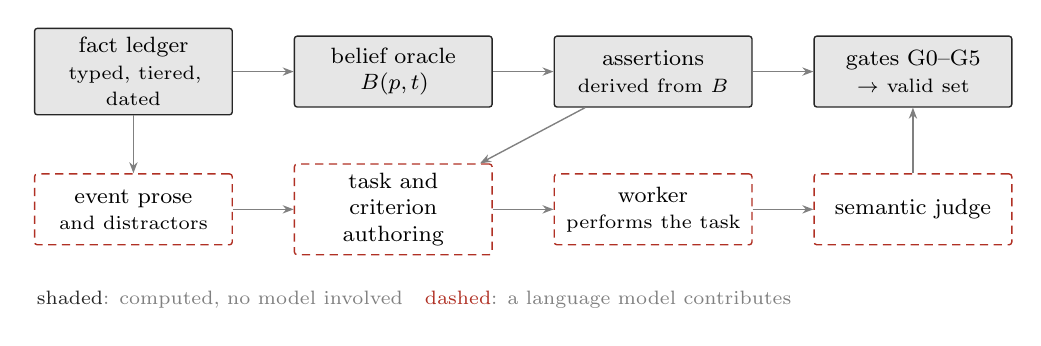
\begin{tikzpicture}[
  font=\footnotesize,
  box/.style={draw=ink, line width=.5pt, rounded corners=1pt, align=center,
              minimum height=9mm, inner xsep=3pt, text width=23mm},
  pure/.style={box, fill=pale!45},
  gen/.style={box, fill=white, draw=accent, densely dashed},
  ar/.style={-{Stealth[length=4pt]}, draw=mid, line width=.5pt},
]
\node[pure] (led) at (0,1.75)    {fact ledger\\\scriptsize typed, tiered, dated};
\node[pure] (b)   at (3.3,1.75)  {belief oracle\\$B(p,t)$};
\node[pure] (asn) at (6.6,1.75)  {assertions\\\scriptsize derived from $B$};
\node[pure] (gate)at (9.9,1.75)  {gates G0--G5\\\scriptsize $\rightarrow$ valid set};

\node[gen] (ev)   at (0,0)       {event prose\\\scriptsize and distractors};
\node[gen] (task) at (3.3,0)     {task and criterion\\authoring};
\node[gen] (work) at (6.6,0)     {worker\\\scriptsize performs the task};
\node[gen] (jud)  at (9.9,0)     {semantic judge};

\draw[ar] (led)  -- (b);
\draw[ar] (b)    -- (asn);
\draw[ar] (asn)  -- (gate);
\draw[ar] (led)  -- (ev);
\draw[ar] (ev)   -- (task);
\draw[ar] (task) -- (work);
\draw[ar] (work) -- (jud);
\draw[ar] (asn)  -- (task);
\draw[ar] (jud)  -- (gate);

\node[font=\scriptsize, text=mid, anchor=west, align=left] at (-1.35,-1.15)
  {\textcolor{ink}{shaded}: computed, no model involved\quad
   \textcolor{accent}{dashed}: a language model contributes};
\end{tikzpicture}
\caption{The two lanes. Everything that decides what is \emph{true} runs along
the shaded row and contains no language model: $B(p,t)$ is a pure function
over the ledger and the event index, and assertions are derived from it.
Models write the prose of an event, author the task and the criteria, perform
the work, and judge the output. Only the first lane can be made model-free;
Table~\ref{tab:entry} is what we did about the rest.}
\label{fig:pipeline}
\end{figure}

\begin{table}[tb]
\centering
\small
\begin{tabular}{@{}r >{\raggedright\arraybackslash}p{34mm} >{\raggedright\arraybackslash}p{27mm} >{\raggedright\arraybackslash}p{45mm}@{}}
\toprule
& stage & can it be removed? & what we did\\
\midrule
1 & world generation & \textbf{yes, from truth} & model writes prose, the ledger decides facts (\S3.1)\\
2 & task authoring & no & pinned, then screened per item (\S4)\\
3 & criterion authoring & no & pinned, kept out of the judge's family (\S5.1)\\
4 & task execution & no, it \emph{is} the measurement & pin the model \emph{and} the harness (\S6.1--6.2)\\
5 & scoring & partly & programmatic where measured to be better (\S3.4)\\
6 & validating the scorer & \textbf{no, and this is the trap} & human anchor, stratified by criterion kind (\S6.3--6.4)\\
\bottomrule
\end{tabular}
\caption{The six places a language model enters, and the verdict at each.
Stage 1 is where most pipelines take the cheap option, asking a model to
produce a scenario \emph{and} the answer to a question about it; the answer is
then true by assertion and no disagreement about it can be adjudicated.}
\label{tab:entry}
\end{table}

Only stage 1 came out clean. Making the ledger primary costs a schema, a
planner and a linter.

Stage 6 is the trap, and it is the one we walked into. When a language model
scores your benchmark \cite{judge} the instinct is to validate the scorer, and
the two cheap ways to do that are an adversarial audit, which feeds it deliberately
wrong outputs and counts false accepts, and a panel, which asks several models
and checks that they agree. Both measure the scorer through the same lens as
the scoring. Both inherit the distribution of whatever you fed them. Sections
6.3 and 6.4 are what that cost us.

\section{Architecture}

\subsection{Ground truth is computed, not asserted}

The generator runs in two passes, and they are never allowed to merge. A fact
planner instantiates scenario archetypes into ledger records: typed
(preference, decision, working rule, reference, outcome, procedure,
commitment, relationship), tiered (personal, team, project, org, external),
with a visibility class, an authority pair of role and capacity, a validity
interval with supersession links, and an explicitness class. An event realizer
then renders those records into naturalistic email, chat, meeting notes and
documents, along with distractors.

The realizer writes every word a system under test ever sees and has no
authority over what is true. The ledger induces
\[
B(p,t) = \{\,\text{facts visible to, valid for, and applicable by principal
$p$'s agent at time $t$}\,\},
\]
a pure function over the ledger and the event index, and every assertion is
derived from it. There is no path from a model's output to a ground-truth
value, so a disagreement about whether an item is correctly keyed is a
question about the ledger and the visibility rules, and can be settled by
reading them. What a model contributes downstream of the ledger is wording:
the prose of an event, and the phrasing of an assertion whose value the ledger
already fixed.

A release-blocking linter enforces the consistency the split makes possible:
ledger-to-event round-tripping of every fact marker, visibility consistency,
interleaving checks, a noise floor, and canary strings for later
training-data-leakage detection \cite{gsm1k}. It runs green across five
organizations and their twins.

\subsection{Salience parity is a construction invariant}

A generated stream leaks. Facts that matter get written more prominently than
distractors, because the model writing them knows which ones matter, and a
system under test can then find them without doing the work the benchmark
claims to measure.

The tempting fix is to re-render until a leak detector goes quiet. That is
fitting the detector, and it produces a stream that passes your checks and
nobody else's. The fix that holds makes parity a property of construction:
distractor type and capacity mirror the probed mix, canonical lengths are
pinned to the probed distribution, counterfactual text is pinned to the base
word count, and positions are enforced mechanically by extracting every fact
and reinserting it at class-stratified band centres.

Measured: one isolated adversarial rater per seed, blinded, scored 58/100 at
$p = 0.067$ against a bar of 65\%. Seed 3 shows a repeatable single-seed
signal at roughly 70\% single-rater accuracy, attributed to subject-shape and
topic-domain residue. We documented that residual and did not chase it.

\subsection{The counterfactual twin makes an item self-falsifying}

Every probe is generated twice (Figure~\ref{fig:twin}). The twin runs against
an alternate ledger in which the probed fact differs, and the two streams are
byte-identical everywhere else. An instance is credited only when both sides
behave correctly, which is to say only when behaviour depends on the fact
under test.

\begin{figure}[tb]
\centering
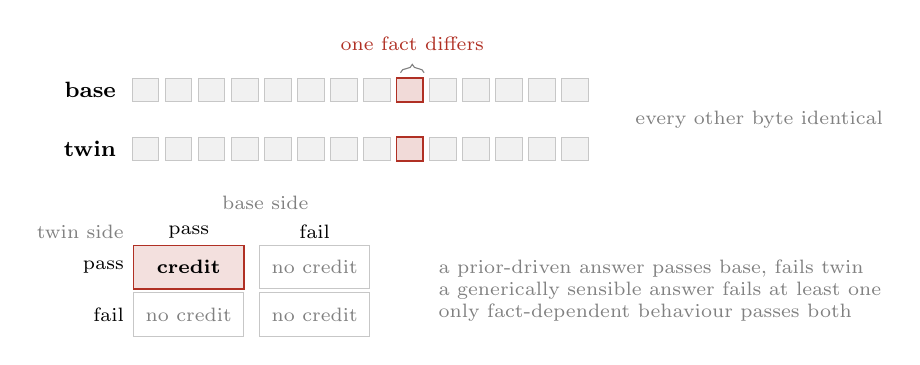
\begin{tikzpicture}[
  font=\footnotesize,
  ev/.style={draw=pale, fill=pale!25, minimum width=3.4mm, minimum height=3mm,
             inner sep=0pt, line width=.3pt},
  delta/.style={draw=accent, fill=accent!18, minimum width=3.4mm,
                minimum height=3mm, inner sep=0pt, line width=.6pt},
]
\node[anchor=east, font=\footnotesize\bfseries] at (-0.25,1.5) {base};
\node[anchor=east, font=\footnotesize\bfseries] at (-0.25,0.75) {twin};
\foreach \i in {0,...,13}{
  \pgfmathsetmacro{\x}{\i*0.42}
  \ifnum\i=8
    \node[delta] at (\x,1.5) {};
    \node[delta] at (\x,0.75) {};
  \else
    \node[ev] at (\x,1.5) {};
    \node[ev] at (\x,0.75) {};
  \fi
}
\draw[decorate, decoration={brace, amplitude=3pt}, draw=mid]
  (3.24,1.72) -- (3.54,1.72);
\node[font=\scriptsize, text=accent, anchor=south] at (3.39,1.88)
  {one fact differs};
\node[font=\scriptsize, text=mid, anchor=west] at (6.1,1.13)
  {every other byte identical};

% credit table
\begin{scope}[shift={(0,-1.55)}]
\node[font=\scriptsize, anchor=east, text=mid] at (-0.15,1.25) {twin side};
\node[font=\scriptsize, anchor=west, text=mid] at (0.85,1.62) {base side};
\node[font=\scriptsize] at (0.55,1.25) {pass};
\node[font=\scriptsize] at (2.15,1.25) {fail};
\node[font=\scriptsize, anchor=east] at (-0.15,0.8) {pass};
\node[font=\scriptsize, anchor=east] at (-0.15,0.2) {fail};
\node[draw=accent, fill=accent!15, line width=.6pt, minimum width=14mm,
      minimum height=5.5mm, font=\scriptsize] at (0.55,0.8) {\textbf{credit}};
\node[draw=pale, line width=.4pt, minimum width=14mm, minimum height=5.5mm,
      font=\scriptsize, text=mid] at (2.15,0.8) {no credit};
\node[draw=pale, line width=.4pt, minimum width=14mm, minimum height=5.5mm,
      font=\scriptsize, text=mid] at (0.55,0.2) {no credit};
\node[draw=pale, line width=.4pt, minimum width=14mm, minimum height=5.5mm,
      font=\scriptsize, text=mid] at (2.15,0.2) {no credit};
\node[font=\scriptsize, text=mid, anchor=west, align=left] at (3.6,0.5)
  {a prior-driven answer passes base, fails twin\\
   a generically sensible answer fails at least one\\
   only fact-dependent behaviour passes both};
\end{scope}
\end{tikzpicture}
\caption{The counterfactual twin and pair credit. Because the streams differ
by one fact and nothing else, an instance is credited only when behaviour
tracks that fact. This closes the two failure modes careful item authoring
does not: answering from parametric knowledge of how organizations usually
work, and producing output generic enough to satisfy whichever side is scored
alone.}
\label{fig:twin}
\end{figure}

Twins are also where construction breaks, and two rules came out of
adjudicating the failures. Never pair a retraction counterfactual with a task
that demands the positive value: if the base task says ``state the required
home for notes'' and the counterfactual says any format is acceptable, the
twin worker cannot comply and the pair is structurally invalid, which was the
dominant drop class on seed 3 at five clusters. And a counterfactual must
invert the aspect the task actually elicits, not merely differ from the base;
the discrimination gate of \S5.3 exists to catch the ones that do not.

\subsection{Criterion kinds, and why the detector choice was measured}

Assertions come in three kinds, and the kind turns out to determine both what
a criterion can catch and how the scorer fails on it. \code{fact\_applied}
asks that the output use the correct fact. \code{scope\_correct} asks that it
respect tier, authority and precedence. \code{fact\_absent} asks that it
\emph{not} use a fact it should not have: stale, superseded, out of scope, or
never witnessed. Leakage and staleness live in the third kind.

The first design scored applied content with authored regular expressions, on
the principle that programmatic scoring beats a model wherever it can reach.
We measured that instead of assuming it. On ceiling runs, where the worker
held the correct facts and was demonstrably right, the regex assertions failed
39--42\% of runs against 9--17\% for semantic checking of the same content
(Figure~\ref{fig:detector}). Paraphrase defeats the pattern. Applied-content
assertions moved to semantic-always in probe-spec v0.3, and that is how a
language model got into the scoring path.

\begin{figure}[tb]
\centering
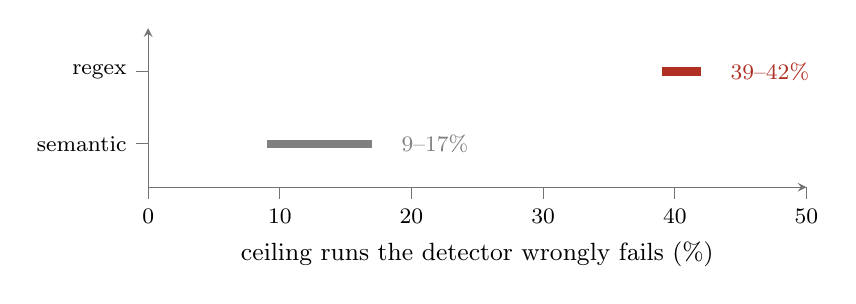
\begin{tikzpicture}
\begin{axis}[
  tufte,
  width=.82\textwidth, height=3.6cm,
  xmin=0, xmax=50,
  xlabel={ceiling runs the detector wrongly fails (\%)},
  ytick={0,1}, yticklabels={semantic, regex},
  ymin=-0.6, ymax=1.6,
  xtick={0,10,20,30,40,50},
  clip=false,
]
\addplot[draw=mid, line width=3pt, mark=none] coordinates {(9,0) (17,0)};
\addplot[draw=accent, line width=3pt, mark=none] coordinates {(39,1) (42,1)};
\node[font=\footnotesize, text=mid, anchor=west] at (axis cs:18.5,0) {9--17\%};
\node[font=\footnotesize, text=accent, anchor=west] at (axis cs:43.5,1) {39--42\%};
\end{axis}
\end{tikzpicture}
\caption{Why applied-content scoring is semantic. On ceiling runs, where the
worker was handed the correct facts and was demonstrably right, authored regex
assertions failed 39--42\% of runs against 9--17\% for semantic checking of
the same content. A detector that fires on two-fifths of correct answers is
not a detector.}
\label{fig:detector}
\end{figure}

\subsection{Three rules that came out of adjudication}

Each was written after a specific defect class was identified, applied
uniformly to every organization the day it was written, and carried with
before-and-after counts.

\textbf{Co-valid siblings are never punished.} In tier-collision scenarios the
personal, team and org facts often complement rather than conflict, so an
assertion demanding one be absent punishes a correct output. The tier rule for
sibling guards removed 168 assertion pairs across five organizations.

\textbf{Criteria describe observable artifacts, not authorial intent.} Forty
criteria phrased as pure retractions were rewritten as observable absence in
the artifact the task produces, after a classifier sweep plus a hand audit.
This is the class that produced the unnatural-negation defects, and rewriting
them recovered five clusters on seed 2.

\textbf{Repairs keep task text byte-identical.} Every criterion repair leaves
the prompt the worker sees unchanged, verified by a prompt-equality check per
seed, so cached worker outputs stay valid and a repair cannot smuggle in an
easier task. That is what made criterion repair affordable under the quota.

\section{Screening: an item is not valid until it is measured to be}

Screening asks, of every probe, two questions you can only answer by running
the thing. Does a worker with no memory fail it? Does a worker handed exactly
the right facts pass it? An item that the oracle fails measures reasoning
rather than memory. An item the memoryless floor passes measures priors, which
is the confound a controlled baseline is there to expose \cite{memdelta}. We
record per-side guessability with every item. Seed 1 carries a mean of 0.33,
and seven surviving clusters sit at 1.0; those are disclosed cluster by
cluster, and they survive only because pair credit still requires the twin
side.

We fixed the gate unit before the evidence existed, which matters more than
which unit we picked. We gate on \emph{instances}, not clusters, and a cluster
survives when at least two of its three instances are valid. A cluster-level
reading would have failed differently, and the stricter all-instances rule
needs per-run reliability above 98\%, which nothing in this pipeline delivers.

Screening is the expensive part. One seed costs 486 worker runs, against a
quota where one credit pack buys roughly a thousand at the pinned model and
effort. Three seeds were screened and two withheld unscreened as holdouts, and
the byte-identical rule of \S3.5 is what keeps criterion repair inside that
budget.

The outcome is reported as measured (Table~\ref{tab:gates}), and the companion
paper reports the same gates first, with the per-seed adjudication behind them
\cite{companion}. All three instance gates fail. Seed 3's cluster gate also fails. The shortfall is
structured, not random. It is the twin-anchoring residual of \S3.3, the same
defect family that drives the cluster drops.

\begin{table}[tb]
\centering
\small
\begin{tabular}{@{}l r r l l@{}}
\toprule
seed & clusters surviving & valid instances & instance gate ($\geq$135) & cluster gate ($\geq$45)\\
\midrule
1 & 46/54 & 125 & \textbf{FAIL} & pass\\
2 & 46/54 & 131 & \textbf{FAIL} & pass\\
3 & 40/54 & 115 & \textbf{FAIL} & \textbf{FAIL}\\
\midrule
\multicolumn{2}{@{}l}{total valid paired instances} & \textbf{371} &
\multicolumn{2}{l}{A1 50 \quad A2 43 \quad A4 106 \quad A7 172}\\
\bottomrule
\end{tabular}
\caption{Screening outcome, carried as measured. No probe that failed a gate
was repaired to recover it, no criterion was rewritten after seeing that it
cost an instance, and no threshold moved once it bound. A gate relaxed once it
binds was never a gate.}
\label{tab:gates}
\end{table}

\section{The quality apparatus, including the parts that did not work}

\subsection{Blinding, enforced by code and not by the spec}

Semantic verdicts go through an export step that assigns opaque row and
criterion identifiers; the judge never sees conditions, sides, or which
organization a row belongs to. The spec required blinding from the start. We
\emph{implemented} it on 2026-07-25, after reading the export format against
the spec and finding that it enforced nothing. We kept the earlier unblinded
pass in git; it agrees with the blinded one at 97.6\%, 26 flips of 1,092, 14
true-to-false against 12 false-to-true. A stated rule that no code enforces is not a rule.

\subsection{The scorer-exploit audit, which still reads FAIL}

Attacking your own scorer with degenerate outputs is standard advice
\cite{abc}. We judged four degenerate output types blind against the real
criteria: an empty output, a waffle that commits to nothing, an output that
enumerates both values, and a correct base output as control. The first audit,
run on 45 pairs before any cross-side absence detector existed, found the
enumerate-both-values hedge earning full pair credit on 27 of them, and 18 still
did after mechanical detectors were added. On the frozen canon, 46 pairs per
type, every degenerate type scores zero pair-passes.

The prespecified bar nonetheless still reads FAIL, on three waffle
counterfactual sides scoring 1.0. All three are absence-only sides, which are
passable by content-free output by construction while the pair still fails.
Re-scoping the single-side clause to sides carrying positive content gives
PASS. Both readings live in the artifact permanently, and the re-scope carries
a post-hoc label. A bar rewritten after it bites is not a bar.

\subsection{A detector layer, measured and discarded the same day}

We built generated semantic cross-side detectors to catch outputs that satisfy
their own side's criteria while also satisfying the twin's. Measured against
honest instances, they flipped 19 and caught zero true positives. We rejected
the layer and committed the adjudication. Keeping a negative result in the
repository costs nothing and is the only way a later reader can tell that the
absence of a feature was a decision rather than an oversight.

\subsection{The bug a control caught}

The judge-panel scorer of \S6.4 keyed verdicts by (run, assertion). Run
identifiers repeat across organizations, so the second organization silently
overwrote the first and $\kappa$ came out 0.399 instead of 0.537. What caught
it was a control asserting that the v1 baseline must recompute to $n=150$, raw
0.813, $\kappa$ 0.537. The scorer now refuses to emit a report unless that
control passes.

\section{Five model dependencies we could not remove}

\subsection{The worker}

Under identical strict rules, 37 of 54 probe clusters survive the ceiling gate
for gpt-5.4 and 17 of 54 for gpt-5.4-mini, a smaller model of the same family
(Figure~\ref{fig:pins}, left; the screening run is the companion paper's
\cite{companion}). Nothing about the probes changed between those
numbers. A valid item is therefore not a property of the item. It is a
property of the pair, item and worker, and a released valid set is defined
relative to the model that screened it. Any benchmark that decides which of
its items are answerable by checking whether a model can answer them inherits
this, whether or not it says so, and it is one reason two benchmarks aimed at
the same capability can rank the same models differently \cite{benchbench}. We
handle it by pinning the worker, reporting
the pin wherever a number appears, and publishing the per-worker re-screening
procedure.

\subsection{The harness}

Before admitting a second agent harness to any protocol path we ran a
prespecified equivalence study, reported in full in the companion paper
\cite{companion}: 60 runs, 20 per condition, acceptance rule
written into the protocol file before any run at 90\% outcome agreement per
condition. The two harnesses ran identical weights at identical effort; only
the scaffold differed. The study failed its own rule (Figure~\ref{fig:pins},
right), and the disagreement is not uniform. Where the task is easy to fail or
easy to pass the harnesses agree; on the twin ceiling, which asks a worker to
produce a deliverable consistent with a counterfactual fact while an almost
identical base fact is absent, the same weights behind different scaffolds
disagree on more than a third of outcomes.

The harness is part of the consumer, not a neutral pipe to the weights. A
benchmark that pins a model and not its harness has not pinned its worker.

\begin{figure}[tb]
\centering
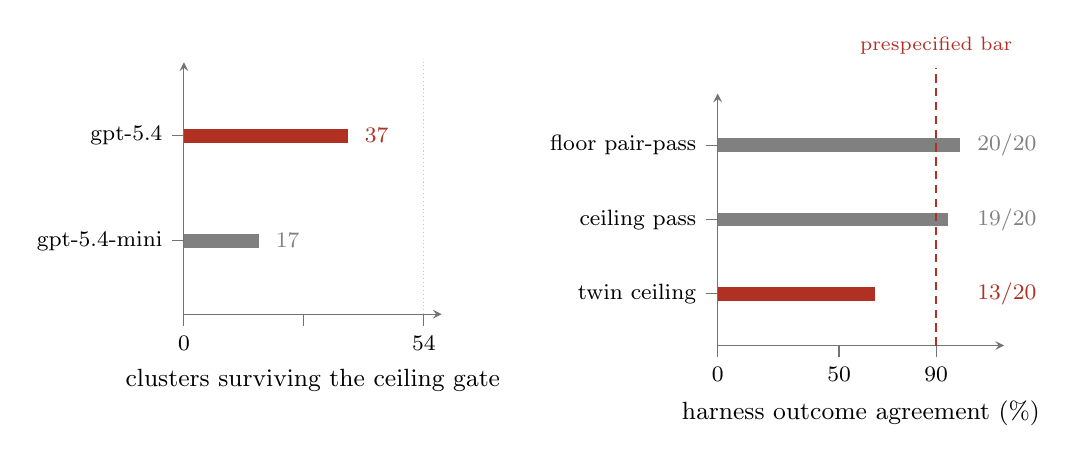
\begin{tikzpicture}
\begin{axis}[
  tufte,
  name=left,
  width=.27\textwidth, height=3.2cm,
  scale only axis,
  xmin=0, xmax=58, xtick={0,27,54}, xticklabels={0,,54},
  xlabel={clusters surviving the ceiling gate},
  ytick={0,1}, yticklabels={gpt-5.4-mini, gpt-5.4},
  ymin=-0.7, ymax=1.7, clip=false,
]
\addplot[draw=mid, line width=5pt] coordinates {(0,0) (17,0)};
\addplot[draw=accent, line width=5pt] coordinates {(0,1) (37,1)};
\node[font=\footnotesize, text=mid, anchor=west] at (axis cs:18.5,0) {17};
\node[font=\footnotesize, text=accent, anchor=west] at (axis cs:38.5,1) {37};
\draw[draw=pale, line width=.4pt, densely dotted]
  (axis cs:54,-0.7) -- (axis cs:54,1.7);
\end{axis}
\begin{axis}[
  tufte,
  at={(left.outer east)}, anchor=outer west, xshift=4mm,
  width=.30\textwidth, height=3.2cm,
  scale only axis,
  xmin=0, xmax=118, xtick={0,50,90}, xticklabels={0,50,90},
  xlabel={harness outcome agreement (\%)},
  ytick={0,1,2}, yticklabels={twin ceiling, ceiling pass, floor pair-pass},
  ymin=-0.7, ymax=2.7, clip=false,
]
\addplot[draw=accent, line width=5pt] coordinates {(0,0) (65,0)};
\addplot[draw=mid, line width=5pt] coordinates {(0,1) (95,1)};
\addplot[draw=mid, line width=5pt] coordinates {(0,2) (100,2)};
\node[font=\footnotesize, text=accent, anchor=west] at (axis cs:103,0) {13/20};
\node[font=\footnotesize, text=mid, anchor=west] at (axis cs:103,1) {19/20};
\node[font=\footnotesize, text=mid, anchor=west] at (axis cs:103,2) {20/20};
\draw[draw=accent, line width=.5pt, densely dashed]
  (axis cs:90,-0.7) -- (axis cs:90,3.05);
\node[font=\scriptsize, text=accent, anchor=south] at (axis cs:90,3.1)
  {prespecified bar};
\end{axis}
\end{tikzpicture}
\caption{The same rules, a different model or a different scaffold. Left:
probe clusters surviving the ceiling gate under identical strict rules, two
models of one family. Right: outcome agreement between two agent harnesses
running identical weights at identical effort, against a bar fixed before any
run. Agreement collapses exactly where the condition is hardest.}
\label{fig:pins}
\end{figure}

\subsection{The judge fails by criterion kind, not in aggregate}

Two checks ran on the judge, one cheap and automated, one expensive and human.
They disagree about whether the judge is sound.

\textbf{The automated audit could not have failed.} Twenty deliberately
wrong-but-topical outputs were judged blind against the real criteria, giving
2 false accepts of 41 as measured and 0 of 39 after adjudicating two criteria
that an under-specified decoy legitimately satisfied. Read alone this says the
judge does not accept plausible-sounding wrong answers. Resolving those 41
criteria back to their kinds shows why the reading was premature: 30 were
\code{fact\_applied}, 11 were \code{scope\_correct}, and \emph{none} were
\code{fact\_absent}. A decoy is built by stating wrong values, so it exercises
criteria demanding content; a criterion phrased as absence is satisfied by an
output that never raises the topic, so a decoy cannot probe it without being
built differently. The audit was structurally incapable of detecting a failure
on absence criteria, which is exactly where the failure was.

\textbf{The human check failed the gate.} A blinded 150-pair packet rated
against the committed judge verdicts, an anchor the companion paper reports
first \cite{companion}, gives raw agreement 0.813 at $\kappa = 0.537$, against
a prespecified $\kappa \geq 0.75$. A percentile bootstrap over the 89 fact
clusters the packet spans, 10,000 replicates at a fixed seed with no
degenerate replicate, puts the 95\% interval at [0.370, 0.688]. Clusters are
the resampling unit because the packet is stratified with a per-cluster cap,
and a bootstrap rather than a Wald interval because a normal approximation is
not safe at this count \cite{bowyer, miller}. The upper bound is below the
gate, so the FAIL does not depend on the point estimate. The interval is
post-hoc: the gate was prespecified and measured on the point estimate, and
reporting it is how this paper meets the uncertainty-reporting criterion that
most benchmarks in BetterBench's sample fail \cite{betterbench}.

\begin{table}[tb]
\centering
\small
\begin{tabular}{@{}l r r r r r r l@{}}
\toprule
kind & $n$ & $\kappa$ & hT/jT & hT/jF & hF/jT & hF/jF & direction\\
\midrule
\code{fact\_absent}  & 44 & \textbf{0.166} & 35 & 0 & 8 & 1 & judge over-accepts, every error\\
\code{fact\_applied} & 72 & 0.605 & 40 & 7 & 6 & 19 & mixed\\
\code{scope\_correct}& 34 & 0.561 & 19 & 7 & 0 & 8 & judge under-accepts, every error\\
\midrule
overall & 150 & \textbf{0.537} & \multicolumn{4}{c}{14 disagreements each way} & bias index 0.000\\
\bottomrule
\end{tabular}
\caption{Judge against human, by criterion kind. The aggregate symmetry is a
cancellation, not a property: the judge is one-sidedly permissive on
absence-phrased criteria and one-sidedly strict on scope criteria, and the two
cancel only because this packet happens to hold 44 of the first and 34 of the
second. Bootstrap 95\% intervals on $\kappa$, resampling the same 89 clusters,
are [0.000, 0.493] for \code{fact\_absent}, [0.388, 0.782] for
\code{fact\_applied}, [0.298, 0.837] for \code{scope\_correct} and [0.370,
0.688] overall. A different mix of kinds would not cancel.}
\label{tab:kinds}
\end{table}

Every pair of those intervals overlaps, so they do not establish that $\kappa$
differs by criterion kind, and the claim of this section does not rest on
comparing them. It rests on the direction of the errors and on the
corpus-scale rates. Every one of the 8 disagreements on absence criteria is
the judge accepting where the human rejected, and every one of the 7 on scope
criteria runs the other way: two-sided exact binomial $p = 0.008$ and $p =
0.016$ against an even split, from counts too small to separate three $\kappa$s
but large enough to rule out a coin.

\textbf{The mechanism holds at corpus scale, without human labels.} Joining
all 5,398 committed verdicts to their criterion kind, losslessly and with zero
unmatched identifiers, gives a pooled positive rate of 96.4\% for
\code{fact\_absent} against 39.0\% for \code{fact\_applied} and 36.9\% for
\code{scope\_correct}, holding in every source directory at 93.2--98.9\%. The
memoryless run settles it (Figure~\ref{fig:kinds}). Under a worker that
demonstrably knows nothing, the two content kinds halve and absence does not
move. That is a degenerate pass mode, shown without a single human label and
so without the single-rater limitation.

\begin{figure}[tb]
\centering
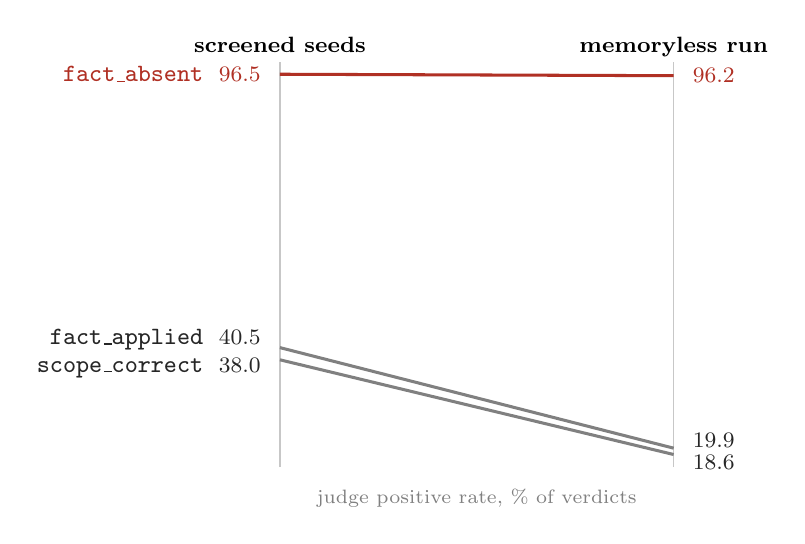
\begin{tikzpicture}[font=\footnotesize]
\def\xa{0}\def\xb{5.0}
\def\sy#1{(#1)*0.062}
\draw[draw=pale, line width=.4pt] (\xa,{\sy{16}}) -- (\xa,{\sy{99}});
\draw[draw=pale, line width=.4pt] (\xb,{\sy{16}}) -- (\xb,{\sy{99}});
\node[anchor=base, font=\footnotesize\bfseries] at (\xa,{\sy{101}}) {screened seeds};
\node[anchor=base, font=\footnotesize\bfseries] at (\xb,{\sy{101}}) {memoryless run};

\draw[draw=accent, line width=1.1pt] (\xa,{\sy{96.5}}) -- (\xb,{\sy{96.2}});
\draw[draw=mid, line width=1.1pt] (\xa,{\sy{40.5}}) -- (\xb,{\sy{19.9}});
\draw[draw=mid, line width=1.1pt] (\xa,{\sy{38.0}}) -- (\xb,{\sy{18.6}});

% labels nudged apart; the lines stay at true positions
\node[anchor=east, text=accent] at ({\xa-0.12},{\sy{96.5}}) {\code{fact\_absent}\ \ 96.5};
\node[anchor=west, text=accent] at ({\xb+0.12},{\sy{96.2}}) {96.2};
\node[anchor=east, text=ink] at ({\xa-0.12},{\sy{40.5}+0.10}) {\code{fact\_applied}\ \ 40.5};
\node[anchor=east, text=ink] at ({\xa-0.12},{\sy{38.0}-0.10}) {\code{scope\_correct}\ \ 38.0};
\node[anchor=west, text=ink] at ({\xb+0.12},{\sy{19.9}+0.10}) {19.9};
\node[anchor=west, text=ink] at ({\xb+0.12},{\sy{18.6}-0.10}) {18.6};
\node[anchor=north, font=\scriptsize, text=mid] at (2.5,{\sy{16}-0.15})
  {judge positive rate, \% of verdicts};
\end{tikzpicture}
\caption{The control that needs no human labels. Moving from the screened
seeds to a memoryless worker halves the positive rate on both content kinds
and leaves absence untouched. Populations: screened seeds $n=1{,}359$ /
$2{,}481$ / $1{,}188$; memoryless run $n=104$ / $196$ / $70$; pooled figures
quoted in the text include the memoryless run and so differ slightly. A
criterion class that does not respond to removing the knowledge under test is
passing by construction.}
\label{fig:kinds}
\end{figure}

\subsection{Judge panels are reliable and jointly invalid}

If one judge is unreliable, the field's reflex is to use several \cite{judge}.
We prespecified a panel before any panel verdict existed: four blinded judges
(haiku-4.5, sonnet-5, opus-5, fable-5.1) re-judging the 478 semantic criteria
on the 146 runs the calibration packet spans, byte-identical batches, verbatim
rubric, no repository access. The committed v1 judge, whose verdicts the packet
was rated against, enters every comparison below as a fifth rater. One panel
member runs the same model as that v1 judge, sonnet-5, so the five raters are
four distinct models, and the panel is a re-run of the model already in the
scoring path plus three others.

They agree with each other, and barely with the human
(Figure~\ref{fig:judges}, left). Five raters give ten judge-to-judge pairs and
five judge-to-human comparisons. Across all ten pairs, judge-to-judge $\kappa$
runs 0.927--0.970 at 0.964--0.985 raw agreement; against the human anchor all
five run $\kappa$ 0.518--0.563. On the 44 sampled absence criteria all four
panel judges produced \emph{byte-identical verdict vectors}, 42 true and 2
false in the same positions, where the committed v1 judge gave 43/1 and the
human gave 35/9. That roster is four models from one vendor's line, one of
them the scorer under test run a second time; it is the diversity a panel
usually means, and it buys nothing on this criterion class, because the
failure is perfectly correlated.

Aggregation cannot repair what is perfectly correlated
(Figure~\ref{fig:judges}, right). Majority vote, unanimous-AND and
unanimous-OR all land at or below the best single judge, and on absence
criteria every rule returns the identical $\kappa = 0.313$, because every rule
is applied to the same vector. The panel is unanimous on 141 of 150 items, and
the human disagrees with that unanimous verdict on 24 of them; restricted to
the unanimous subset $\kappa$ is 0.575, still a clear fail. The direction on
that subset is the same one-sided pattern as before: 7 of 7 panel over-accepts
on absence, 6 of 6 under-accepts on scope.

Test-retest closes the remaining alternative, and the sonnet-5 arm is what
supplies it. A fresh run of the model behind the committed v1 judge, against
those same committed verdicts, agrees at 0.973, $\kappa$ 0.944 over the 478
exported criteria. That arm is therefore doing two jobs: it is one of the ten
judge-to-judge pairs, and it is a reliability check on the scorer itself
rather than a fifth independent opinion about the outputs. Read as a
reliability check, it says the judge--human gap is not instability. It is a
stable, reproducible divergence.

\begin{figure}[tb]
\centering
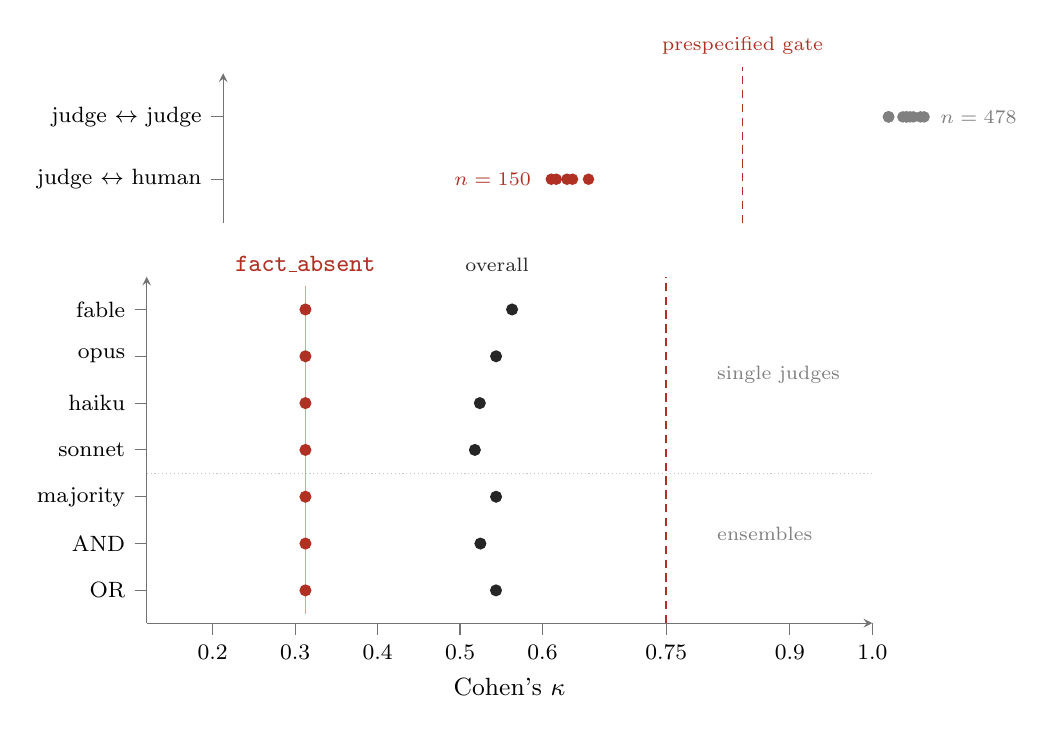
\begin{tikzpicture}
\begin{axis}[
  tufte,
  name=top,
  width=.76\textwidth, height=1.9cm, scale only axis,
  xmin=0.12, xmax=1.0, xtick=\empty,
  axis x line=none,
  ymin=-0.7, ymax=1.7, ytick={0,1},
  yticklabels={judge $\leftrightarrow$ human, judge $\leftrightarrow$ judge},
  clip=false,
]
\addplot[only marks, mark=*, mark size=1.6pt, draw=mid, fill=mid]
  coordinates {(0.9269,1)(0.9270,1)(0.9272,1)(0.9444,1)(0.9486,1)
               (0.9488,1)(0.9531,1)(0.9571,1)(0.9658,1)(0.9701,1)};
\addplot[only marks, mark=*, mark size=1.6pt, draw=accent, fill=accent]
  coordinates {(0.5180,0)(0.5240,0)(0.5370,0)(0.5437,0)(0.5631,0)};
\node[font=\scriptsize, text=mid, anchor=west] at (axis cs:0.978,1) {$n=478$};
\node[font=\scriptsize, text=accent, anchor=east] at (axis cs:0.505,0) {$n=150$};
\draw[draw=accent, line width=.5pt, densely dashed]
  (axis cs:0.75,-0.7) -- (axis cs:0.75,1.8);
\node[font=\scriptsize, text=accent, anchor=south] at (axis cs:0.75,1.85)
  {prespecified gate};
\end{axis}
\begin{axis}[
  tufte,
  at={(top.outer south west)}, anchor=outer north west, yshift=-3mm,
  width=.76\textwidth, height=4.4cm, scale only axis,
  xmin=0.12, xmax=1.0, xlabel={Cohen's $\kappa$},
  xtick={0.2,0.3,0.4,0.5,0.6,0.75,0.9,1.0},
  xticklabels={0.2,0.3,0.4,0.5,0.6,0.75,0.9,1.0},
  ymin=-0.7, ymax=6.7, ytick={0,1,2,3,4,5,6},
  yticklabels={OR, AND, majority, sonnet, haiku, opus, fable},
  clip=false,
]
\addplot[only marks, mark=*, mark size=1.7pt, draw=ink, fill=ink]
  coordinates {(0.5631,6)(0.5437,5)(0.5240,4)(0.5180,3)
               (0.5437,2)(0.5247,1)(0.5436,0)};
\addplot[only marks, mark=*, mark size=1.7pt, draw=accent, fill=accent]
  coordinates {(0.3125,6)(0.3125,5)(0.3125,4)(0.3125,3)
               (0.3125,2)(0.3125,1)(0.3125,0)};
\draw[draw=accent, line width=.4pt, opacity=.45]
  (axis cs:0.3125,-0.5) -- (axis cs:0.3125,6.5);
\node[font=\scriptsize, text=accent, anchor=south] at (axis cs:0.3125,6.6)
  {\code{fact\_absent}};
\node[font=\scriptsize, text=ink, anchor=south] at (axis cs:0.545,6.6) {overall};
\draw[draw=pale, line width=.4pt, densely dotted]
  (axis cs:0.12,2.5) -- (axis cs:1.0,2.5);
\node[font=\scriptsize, text=mid, anchor=west] at (axis cs:0.80,4.6)
  {single judges};
\node[font=\scriptsize, text=mid, anchor=west] at (axis cs:0.80,1.2)
  {ensembles};
\draw[draw=accent, line width=.5pt, densely dashed]
  (axis cs:0.75,-0.7) -- (axis cs:0.75,6.7);
\end{axis}
\end{tikzpicture}
\caption{Reliable, and jointly invalid, on one scale. Five raters, the four
panel judges and the committed v1 judge, give ten pairs and five
human comparisons. Top: all ten judge-to-judge pairs sit far to the right of
the prespecified gate (dashed, at $\kappa=0.75$); not one of the five
judge-to-human comparisons comes near it.
Bottom: $\kappa$ against the human anchor for each single judge and each
aggregation rule. No rule beats the best single judge, and on absence criteria
every rule returns the identical $\kappa=0.313$, a dead-straight column,
because all four panel judges produced the same verdict vector. The aggregation
arm is post-hoc; the panel itself was prespecified. Consensus among
language-model judges is not evidence of validity.}
\label{fig:judges}
\end{figure}

\subsection{The anchor expires on the provider's schedule}

The pinned worker, gpt-5.4 at effort medium behind codex-cli 0.144.5, was
deprecated by its provider on 2026-09-04, mid-pilot, and is unreachable
through any available billing path. Screening cannot be re-run. Comparative
evaluation was cut from the release. The re-anchoring procedure now shipped
with the dataset is a first-hand account rather than a contingency plan, and
it fixes a harness version alongside a model version for the reason in \S6.2.

A pipeline whose valid set is defined relative to a vendor-hosted model needs
the re-anchoring path built and exercised before it is needed. Benchmarks that
plan for decay refresh their items on a schedule they control
\cite{livebench, gsm1k}; a pipeline has to re-anchor its worker on a schedule
it does not. We had written the rule down and never run it. The difference
between those two states is most of the work.

\section{What we would build differently}

This is the part meant to be copied.

\begin{enumerate}[leftmargin=1.5em, itemsep=2pt, topsep=3pt]
\item \textbf{Plan facts before prose.} If a model decides what is true, a
  disagreement between the scorer and the key has no appeal court.
\item \textbf{Screen every item against a memoryless floor and an oracle
  ceiling.} Budget for it. This is not a sanity check; it is the definition of
  a valid item, and 17 of our 54 clusters failed it.
\item \textbf{Pin the harness, not only the model.} A result reported without a
  scaffold version is unanchored, and the disagreement concentrates exactly in
  the conditions you care most about.
\item \textbf{Validate the judge per criterion kind, and build the adversarial
  audit per kind too.} An aggregate false-accept rate, and even an aggregate
  over-accept and under-accept balance, conceals opposite directional failures
  that cancel. Ours cancelled to a bias index of exactly zero.
\item \textbf{Do not treat a panel of models as evidence of validity.} Measure
  their agreement with each other if you like; it will be high, and it will
  tell you nothing about whether they are right. Spend the same budget on
  human labels stratified by criterion kind instead.
\item \textbf{Make every re-analysis reproduce a known number before it reports
  a new one.} This caught a silent cross-organization key collision that had
  moved $\kappa$ by 0.14.
\item \textbf{Write the gate unit and the threshold down, with a date, before
  the evidence exists.} Then carry the failures. Four of ours failed.
\item \textbf{Build the re-anchoring path before the vendor makes you.}
\end{enumerate}

\section{Limitations}

Everything here rests on one pipeline in one domain, with one org shape, one
worker family and one judge family. The panel is four models from a single
vendor, one of them the committed judge run again, so it cannot tell a
property of language-model judges as a class from a property of Anthropic
models. We declared that before running it.

Item difficulty is anchored to a model and to no person. The ceiling condition
is the pinned worker with the facts injected, so a valid item is one that
model can do when handed the answer and cannot do without it, and no human has
attempted the probes at all. \S6.1 reports how far that definition moves when
the model changes; the separate point is that the construct is validated by
design rather than measured against human performance \cite{construct}, and
nothing here bounds what a person would score on the same items.

The human anchor is a single rater who is also an author. A second independent
rater on the same 150-pair packet is being arranged and would separate judge
error from rater error, which is the one thing that would upgrade the reading
of \S6.3 from our best interpretation to a demonstrated fact. Nothing in this
paper waits on it, because \S6.3's corpus-scale control and \S6.4's panel both
establish the mechanism without human labels.

The aggregation analysis in \S6.4 is post-hoc. The panel was prespecified; the
ensemble rules were computed after the panel verdicts existed. It is a
re-aggregation of prespecified measurements, not a new measurement, and it
carries that label wherever it appears.

Judge identity is not mechanically enforced anywhere in the pipeline. The
judge tag is free text and nothing verifies it against the model that ran;
identity rests on the recorded invocation parameter and on nothing else. This
is a real weakness of the instrument, disclosed rather than repaired, and it
is the first thing we would fix in a successor.

Finally, the scorer-exploit audit of \S5.2 still reads FAIL under its literal
prespecified clause, and the re-scoped reading that gives PASS is post-hoc.
Both are reported and neither is withdrawn.

\section{Release}

The dataset is 371 screened paired instances across three simulated
organizations, released CC BY 4.0 with Croissant and RAI metadata, alongside
the screening pipeline, scoring, adapters and release tooling. The generator,
the ledger, probe plans, realization maps, annotated streams, holdout seeds and
rater keys are withheld, because they contain the answers or, in the
generator's case, rebuild them: it is a deterministic function of the seed and
regenerates a holdout ledger's structure exactly. The re-anchoring procedure
ships with the bundle.

This paper takes the dataset as its case and keeps the method
\cite{companion}.

\section*{Acknowledgements}
Harshit Agarwal reviewed an early draft of the gate criteria and the capability
ladder. His work at Boston Consulting Group on organizational structure and how
information moves through it informed the tier and authority model of \S3.1. He
reviewed the measurement design only: he saw no seed content, no fact ledger and
no results, and he is not a rater in any measurement reported in this paper.

\section*{Author contributions}
M.S. designed the benchmark, built the generator, screening and scoring
pipelines, ran every measurement, and wrote the paper. The calibration packet
behind \S6.3 was rated by M.S. alone, which is the single-rater limitation \S8
records and the one this work most needs repaired.

\section*{Competing interests and funding}
This is an independent study with no institutional affiliation and no funding
from any vendor whose system appears in the companion benchmark's inclusion
criteria. No author-affiliated memory system is evaluated anywhere in this work.

\section*{Ethics}
The organizations, people and events in the dataset this paper draws on are
synthetic; no real personal data was collected or processed. The only
human-subject component is the author's own rating of the calibration packet.

\section*{Data and code availability}
The dataset is at \url{https://huggingface.co/datasets/notmehul/memory-bench}
under CC BY 4.0. The harness, the screening and scoring pipeline, and the
evidence behind every number in this paper are at
\url{https://github.com/notmehul/memory-bench} under MIT, and the dated
development record is at \url{https://github.com/notmehul/memory-bench-history}.
Section~9 lists the bundle contents and the withheld material.

% The monospace path below is one unbreakable word and runs 4pt past the
% margin; the \allowbreak marks let it wrap at the underscores instead.
\section*{Reproducibility}
Every number in this paper derives from a committed artifact, and
\code{tests/test\_\allowbreak pipeline\_\allowbreak paper.py} asserts the mapping,
including the figure
coordinates where a typo would otherwise render silently. One limit is
structural: the pinned worker was withdrawn by its provider on 2026-09-04
(\S6.5), so the screening anchors cannot be reproduced under the model that
produced them, and the re-anchoring procedure exists because we had to run it.

\begin{thebibliography}{99}
\footnotesize
\setlength{\itemsep}{0pt}\setlength{\parsep}{0pt}
\bibitem{companion} Srivastava, M. \emph{memory-bench: A Screened Benchmark
Dataset and Validity Study for Organizational Memory in Agent Harnesses}.
Companion preprint, Zenodo, 2026.
DOI: \href{https://doi.org/\companionDOI}{\companionDOI}.
\bibitem{judge} Zheng, L., Chiang, W.-L., Sheng, Y., et al. \emph{Judging
LLM-as-a-Judge with MT-Bench and Chatbot Arena}. arXiv:2306.05685.
\bibitem{construct} Bean, A., Kearns, R., Romanou, A., et al. \emph{Measuring
what Matters: Construct Validity in Large Language Model Benchmarks}.
arXiv:2511.04703.
\bibitem{betterbench} Reuel, A., Hardy, A., Smith, C., Lamparth, M., Hardy, M.,
and Kochenderfer, M. \emph{BetterBench: Assessing AI Benchmarks, Uncovering
Issues, and Establishing Best Practices}. arXiv:2411.12990.
\bibitem{abc} Zhu, Y., Jin, T., Pruksachatkun, Y., et al. \emph{Establishing
Best Practices for Building Rigorous Agentic Benchmarks}. arXiv:2507.02825.
\bibitem{miller} Miller, E. \emph{Adding Error Bars to Evals: A Statistical
Approach to Language Model Evaluations}. arXiv:2411.00640.
\bibitem{bowyer} Bowyer, S., Aitchison, L., and Ivanova, D. \emph{Position:
Don't Use the CLT in LLM Evals With Fewer Than a Few Hundred Datapoints}.
arXiv:2503.01747.
\bibitem{benchbench} Perlitz, Y., Gera, A., Arviv, O., et al. \emph{Do These
LLM Benchmarks Agree? Fixing Benchmark Evaluation with BenchBench}.
arXiv:2407.13696.
\bibitem{gsm1k} Zhang, H., Da, J., Lee, D., et al. \emph{A Careful Examination
of Large Language Model Performance on Grade School Arithmetic}.
arXiv:2405.00332.
\bibitem{livebench} White, C., Dooley, S., Roberts, M., et al. \emph{LiveBench:
A Challenging, Contamination-Limited LLM Benchmark}. arXiv:2406.19314.
\bibitem{locomo} Maharana, A., Lee, D.-H., Tulyakov, S., Bansal, M., Barbieri,
F., and Fang, Y. \emph{Evaluating Very Long-Term Conversational Memory of LLM
Agents}. arXiv:2402.17753.
\bibitem{memdelta} Wang, K. \emph{MemDelta: Controlled Baselines and Hidden
Confounds in Agent Memory Evaluation}. arXiv:2606.29914.
\bibitem{memtrack} Deshpande, D., Gangal, V., Mehta, H., Kannappan, A., Qian,
R., and Wang, P. \emph{MEMTRACK: Evaluating Long-Term Memory and State Tracking
in Multi-Platform Dynamic Agent Environments}. arXiv:2510.01353.
\bibitem{memoryarena} He, Z., Wang, Y., Zhi, C., Hu, Y., et al.
\emph{MemoryArena: Benchmarking Agent Memory in Interdependent Multi-Session
Agentic Tasks}. arXiv:2602.16313.
\bibitem{gatemem} Ren, Z., Yang, Y., Chen, Y., Zhao, Z., et al. \emph{GateMem:
Benchmarking Memory Governance in Multi-Principal Shared-Memory Agents}.
arXiv:2606.18829.
\end{thebibliography}

\end{document}
